\chapter{Linear Regression}
\label{chp:lin_reg}
Regression is a statistical method to model the relation between a set of explanatory variable (i.e features) and a scalar response, also referred to as dependent variable. Therefore, our \textit{sample domain} is $\Xc=\R^d$ and our \textit{response set} is $\Yc=\R$. We assume that there exists some deterministic (unknown to us) function $f:\Xc\rightarrow\Yc$ that is \textit{underlying} the relation between each sample $x$ and it's response $y$.

\begin{figure}[!h]
	\centering
	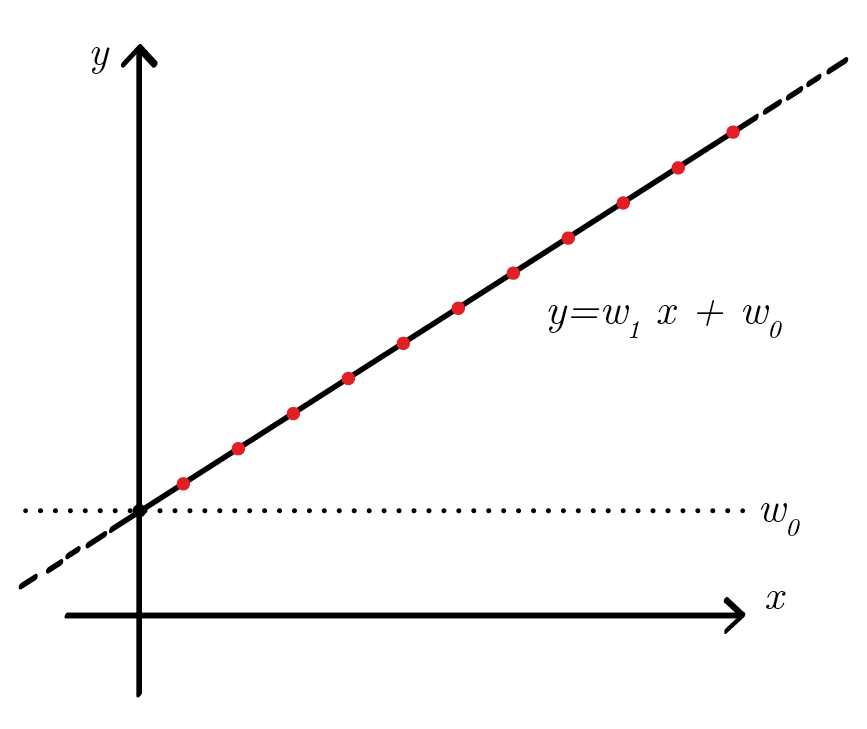
\includegraphics[width=0.5\textwidth]{chapters/intro.regression/figures/2_1.png}
	\caption{\textbf{Linear Regression Illustration:} Illustration of a regression problem with a single explanatory variable. Samples represented with red dots.}
\end{figure}

For reasons we discuss later (\todo{add reference to no free lunch}), whenever we try to model such a relation, we restrict ourselves to specific families of function. These families are referred to as \textit{hypothesis classes}. In the case of linear regression we aim to model the relation using a linear function $f$. Formally, we define hypothesis class of linear regressors as the set of linear functions from the domain set to the response set: 
\begin{equation}\label{eqn:lin_reg_h}
\Hreg\coloneqq\left\{h: h\left(x_1,\ldots,x_d\right)=w_0+\underset{i=1}{\overset{d}{\sum}}x_iw_i,\,\, w_0,w_1,\ldots,w_d\in\R\right\}
\end{equation}
Each function $h$ in the class is characterized by the \textbf{weights} (or regression coefficients) $w_1,\ldots,w_d$ representing the $d$ features and an \textbf{intercept} $w_0$. To simplify notation, for a given sample $\x=\left(x_1,\ldots,x_d\right)^\top \in \R^d$ we add a zero-th coordinate with the value of one, and define $\x=\left(1,x_1,\ldots,x_d\right)^\top \in \R^{d+1}$. Using this notation each function in the hypothesis class can be written in the form $h\left(\x\right)=\left<\x,w\right>=\x^\top w$. From this point onward we will assume that the intercept is already incorporated into the weights vector and samples.
\\
\\
Thus, given a set of samples \trainset also referred to as a \textit{training set}, we are looking for some vector $\w\in\R^{d}$ such that $\forall i\in\left[m\right]\quad y_i=\x^\top_i w$. Let us arrange the data in a matrix form. We define a response \textit{column vector} $\y\in\R^m$ and a samples \textit{matrix} $\X\in\R^{m\times d}$ as follows (where rows represent samples and columns represent features):

$$
\X =
\left[
\begin{array}{ccc}
\horzbar & \x_1 & \horzbar \\
\horzbar & \x_2 & \horzbar \\
		 & \vdots    & \\
\horzbar & \x_m & \horzbar
\end{array}
\right]\quad\quad
\y=\left[\begin{array}{c} y_1 \\ y_2 \\ \vdots \\ y_m \end{array}\right]
$$
The samples matrix $\X$ is referred to as the \textit{design matrix}. Now we can write it as a system of $m$ independent linear equations, which we want to solve for $\w$ (a set of $d$ variables): 
\begin{equation}
\y=\X\w
\label{eqn:lin_reg_model}
\end{equation}

If there exists (at least one) solution, it means that $f$ that created our data is indeed in $\Hreg$. This is called \textbf{The Realizable Case} or \textbf{The Realizability Assumption}. Later in this chapter we will discuss why the assumption that the responses $\y$ are \textit{exactly} linear in the samples $\X$ is not realistic. Many times, even when the relation is indeed linear, the given data may be almost linear. In such cases $f$ is \textit{not} in $\Hreg$. This is called \textbf{The Non-Realizable Case} in which we must settle for finding $\widehat{f}\in\Hreg$ which is "good enough" for our purposes.
\\~\\
In the realizable case, the system of equations has either a unique solution or an infinite number of solutions, depending on the kernel of $\X$ being trivial or non-trivial (i.e $dim\left(Ker\left(\X\right)\right)$ equals or not-equals to zero). As there exists a solution, we know that $\y\in Im\left(\X\right)$. In the case of a trival kernel we conclude that the columns of $X$, meaning the features of our data, are linearly independent. In the non-realizable case, the system has no solution and therefore $\y\not\in Im\left(\X\right)$.



\section{Ordinary Least Squares}
\subsection{Least Squares Loss Function} %TODO - better explanation of risk vs. loss and the empirical risk..
To design a learning algorithm that will learn (predict) $f$, we would like to be able to quantify the \textit{risk} of choosing any predictor $\widehat{f}\in\Hreg$. We derive different algorithms, each with different properties, by the choice of the risk function. In the case of Ordinary Least Squares, OLS, we choose to work with the mean squared risk \eqref{eqn:mse}: 

$$
\left.\begin{array}{c}
\theta \coloneqq \y\\
\widehat{\theta} \coloneqq \widehat{\y}
\end{array}\right\} \Rightarrow R\left(\y,\widehat{\y}\right)=\E_{\widehat{\y}}\left[\left(\y-\widehat{\y}\right)^2\right]
$$

where $\widehat{\y}$ is the linear prediction of $\y$ when selecting some predictor from our hypothesis class: 
$$ \widehat{\y}=\widehat{f}\left(\x\right)=\x^\top\widehat{\w}\quad s.t \quad \widehat{\w}\in \Hreg $$
As we assess our chosen hypotheses using the squared risk it makes sense to choose $\widehat{f}$ that minimizes the same loss \textit{on the training data we already have}. The function chosen to calculate the risk over a given dataset is called a \textbf{Loss Function} and is denoted by $L_S\left(\widehat{f}\right)$ where $S$ is the set of samples $\widehat{f}$ is evaluated over.

Putting it all together, given a training set \trainset and some prediction rule $\widehat{f}\in\Hreg$ the quantity of the squared risk over the training data is called the \textbf{empirical risk}. In our case the empirical risk of the linear function is given by: $$ R\left(y,\widehat{f}\left(\x\right)\right)=\sum^m_{i=1}\left(y_i-\x_i^\top\widehat{\w}\right)^2 = \norm{\y-\X\widehat{\w}}^2_2=\left(\y-\X\widehat{\w}\right)^\top \left(\y-\X\widehat{\w}\right)$$

\subsection{Residual Sum of Squares}\label{rss}
Therefore, under the selection of the squared risk function, minimizing the empirical risk means minimizing the sum of squares of the deviations of the responses from a linear function. In other words, we choose the linear function in $\Hreg$ that is closest to the responses in terms of the Euclidean distance. The deviation $y_i-\x_i^\top\w$ is called the $i$-th \textbf{residual}. The total empirical risk is therefore called \textbf{Residual Sum of Squares} (or \textbf{RSS}), denoted by:

\begin{align}
RSS\left(\w\right) \coloneqq \norm{\y-\X\w}^2
\label{eqn:rss}
\end{align}

As such, learning the lienar function by ERM is solving the quadratic problem:
\begin{align}
\w^*\coloneqq\underset{\w\in\R^d}{argmin}\,RSS\left(\w\right)=\underset{\w\in\R^d}{argmin}\,\norm{\y-\X\w}^2
\label{eqn:opt_rss}
\end{align}
It is therefore a smooth function of $\w$ with a minimum (or minima) If $X$ is of full rank then $\norm{\y-\X\w}^2$ has a unique minimum. This minimum is the predictor $\widehat{f}$ we would like to find.


\begin{figure}[H]
	\centering
	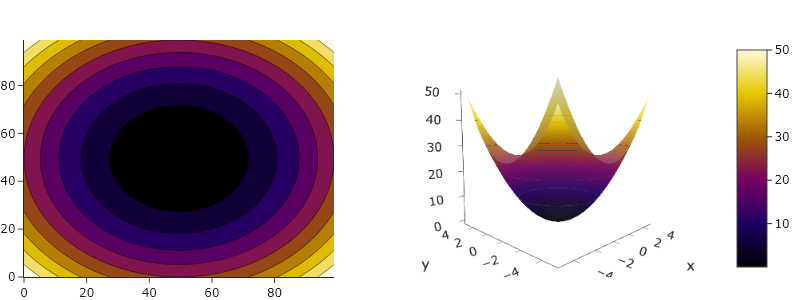
\includegraphics[width=0.7\textwidth]{chapters/intro.regression/figures/rss.png}
	\caption{Illustration of the RSS function in $R^2$ for $X$ of full rank. \GitChapterTwoExamples}
\end{figure}

For $\w$ to be a minimizer of the $RSS$ function all its partial derivatives should be zero. Recalling the definition of the inner product, this condition can be written as: 
$$
\begin{array}{c}
\frac{\partial}{\partial \, w_j}RSS\left(\w\right)=-2\sum^m_{i=1}\left(\x_i\right)_j\cdot\left(y_i-\x_i^\top\w\right)=0\quad j=0,\ldots,d 	\\
\Downarrow	\\
\nabla RSS\left(\w\right)=-2\X^\top\left(\y-\X\w\right)=0	\\
\end{array}
$$


\subsubsection{The Normal Equations}
So a necessary condition for $\w$ to be a minimizer of the objective is to be a solution for the following linear system, known as the \textbf{Normal Equations}:
\begin{equation}
\X^\top\left(y-\X\w\right)=0 \quad \iff \quad \X^\top\y=\X^\top X\w
\label{eqn:normal_eq}
\end{equation}

Let us show that $\widehat{\w}=\left[\X^\top\X\right]^{-1}\X^\top\y$ is the desired minimizer. Before proving so we will first make an assumption over our data $\X,\y$. We will assume that the different features (i.e columns of $\X$) are linearly independent. We will make this assumption in all of the models we will discuss in the course.

~\\\begin{theorem}[The Non-Singular Case]
	Let $\X$ be a design matrix with $m$ observations and $d$ explanatory variables, and $\y$ a response vector. If $d \leq m$ then $\widehat{\w}=\left[\X^\top\X\right]^{-1}\X^\top\y$ is a unique minimizer of \eqref{eqn:opt_rss}. That is, for any $\w\neq\widehat{\w}\quad \norm{\y-\X\w}> \norm{\y-\X\widehat{\w}}$
\end{theorem}
\begin{proof}
As we would like to find a minimizer of the objective, we begin with equating the objective's derivative to zero:
$$
\frac{\partial RSS\left(\w,\X,\y\right)}{\partial \w_{k}}=\frac{\partial\left(\sum_{i=1}^{m}\left(\y_{i}-\x_{i}^{\top}\w\right)^{2}\right)}{\partial \w_{k}}=-2\sum_{i=1}^{m}\left(\y_{i}-\sum_{j=1}^{d}\x_{ij}\w_{j}\right)\x_{k}=0
$$
Equivalently, in matrix notation we get that:
$$
\forall k\in\left[d\right]\quad\left[\X^{\top}\y\right]_{k}-\left[\X^{\top}\X\w\right]_{k}=0\quad\Longrightarrow\quad \X^{\top}\y=\X^{\top}\X\w
$$
	
As $d\leq m$ the design matrix $\X$ is of full column rank $rank\left(\X\right)=d$ and therefore has a trivial kenel. As such, $\X^\top\X$ too is of full rank. This means that the matrix $\X^\top\X$ is non-singular (i.e invertible) and $\left[\X^\top\X\right]^{-1}$ exists:
$$
\begin{array}{c}
\X^{\top}\y=\X^{\top}\X\w\\
\Downarrow\\
\left[\X^{\top}\X\right]^{-1}\X^{\top}\y=\left[\X^{\top}\X\right]^{-1}\X^{\top}\X\w\\
\Downarrow\\
\widehat{\w}=\left[\X^{\top}\X\right]^{-1}\X^{\top}\y
\end{array}
$$

Lastly, we would like to show that $\w$, which we have found to be an extramum of the objective, is a minimum. Taking the second derivative with respect to the parameters:
$$
\frac{\partial^{2}RSS\left(\w,\X,\y\right)}{\partial \w_{k}\partial \w_{l}}	=\frac{\partial-2\sum_{i=1}^{m}\left(\y_{i}-\sum_{j=1}^{d}\x_{ij}\w_{j}\right)\x_{k}}{\partial \w_{l}}
=2\sum_{i=1}^{m}\x_{k}\x_{l}
=2\left[\X^{\top}\X\right]_{kl}\quad\forall k,l\in\left[d\right]
$$

Notice that the matrix $\X^\top\X$ is a positive semi-definite matrix. Now, as we assumed that the columns of $\X$ are independent then for any $v\neq 0$ it holds that $v^\top \left[\X^\top \X\right]v=\left(\X v \right)^{\top} \X v = \norm{\X v}^2>0$ and $\X^\top\X$ is a positive definite matrix. Thus, $\widehat{\w}$  is indeed a minima of the RSS as requested.
\end{proof}

~\\In the case where $d>m$ the null space of $\X^\top\X$ is not trivial. Therefore the matrix is not invertible and there is an inifinite number of solutions. 
~\\
\begin{definition}
	Let $\X\in\R^{m\times d}$ and let $U\Sigma V^\top$ be its SVD. The \textbf{Moore-Penrose pseudoinverse} of $\X$ is $\X^\dagger=V\Sigma^\dagger U^\top$ where $\Sigma^\dagger$ is a $d\times m$ diagonal matrix defined by: $$ \Sigma^\dagger_{i,i}=\begin{cases} 1/\Sigma_{i,i} & \Sigma_{i,i}\neq 0 \\ 0 & \Sigma_{i,i}=0 \end{cases} $$
\end{definition}

\begin{theorem}[The Singular Case]
	Let $\X$ be a design matrix with $m$ observations and $d$ explanatory variables, and $\y$ a response vector. If $d>m$ then $\widehat{\w}=\left[\X^\top\X\right]^{-1}\X^\top\y$ is a unique minimizer of \eqref{eqn:opt_rss}
\end{theorem}
\begin{proof}
	As there are an infinite number of solutions let us begin with finding at least one. Let $\X=U\Sigma V^\top$ be the SVD of matrix $\X$. Therefore, $U,V$ are orthogonal matrices and $\Sigma$ is a $d\times m$ diagonal matrix where the diagonal elements $\Sigma_{i,i}\equiv\sigma_i,\quad \sigma_1\geq\ldots\geq\sigma_d\geq 0$ are the singular values of $\X$.
	
	Let $\Sigma^\dagger$ be a $d\times m$ diagonal matrix such that: 
	$$ \Sigma^\dagger_{i,i} = 
	\begin{cases}
	1/\sigma_i & \sigma_i > 0\\
	0 & \sigma_i = 0\\
	\end{cases} 
	$$
	
	Notice that $\Sigma^\dagger \Sigma$ is too a diagonal matrix and if $\sigma_d>0$ then $\Sigma^\dagger \Sigma=I_d$. Using $\X$'s SVD:
	$$\begin{array}{rcl}
		\X^{\top}\X\w & = & \X^{\top}\y \\
		\left(U\Sigma V^\top\right)^\top \left(U\Sigma V^\top \right)\w & = & \left(U\Sigma V^\top\right)^\top\y\\
		V\Sigma^\top U^\top U\Sigma V^\top\w & = & V\Sigma^\top U^\top \y \\
		\Sigma V^\top \w & = & U^\top\y \\
		\Sigma^\dagger \Sigma V^\top\w & = & \Sigma^\dagger U^\top \y \\
	\end{array}$$
	
	Therefore the solution is: $$ \widehat{\w} = \left(U\left(\Sigma^\dagger\right)^\top V^\top\right)^\top\y = U\Sigma^\dagger V^\top \y = {X^\dagger}^\top \y $$ 
\end{proof}


\begin{corollary}$\widehat{\w}=\left[\X^\top\X\right]^{-1}\X^\top\y$ is always a solution of the Normal Equations\end{corollary}

~\\The estimator we found $\widehat{\w}$ is also referred to as the OLS estimator and is often noted as $\widehat{\w}^{OLS}$.

~\\
\paragraph{Neumerical Stability}
Computers don’t calculate over $\R$, they use bits and more specifically they use floating-point arithmetics with very finite precision. A lot of non-trivial knowledge and care are required in order to understand how learning algorithms are actually implemented in software. \textit{Any} learning algorithm comes down to a lot of calculus (e.g gradients) and linear algebra (e.g. inverses) implemented in software. You should care \textit{deeply} about how algorithms are implemented and when they break numerically, as in the following example.

~\\Sometimes $\X^\top\X$ is formally invertible but \textit{close to singular}. This happens if columns of $\X^\top$ are almost co-linear or if one column of $\X^\top$ is almost spanned by other columns. In this case some singular values of $\X$ will be nonzero, but very small. When this happens, Gauss elimination may yield wildly incorrect results. Also, because of double-precision arithmetics, $1/\sigma_i$ will not be precise. The practical solution in such cases is to choose a machine precision threshold, $\eps$ and let: $$ \Sigma^{\dagger,\eps}_{i,i}=\begin{cases} 1/\sigma_i & \sigma_i>\eps \\ 0 & \sigma_i \leq \eps \end{cases} $$

~\\
\begin{example}
	Let us find the OLS estimator over some mock scenario. Suppose we are interested in regressing running times in a $100m$ on an athlete's height and weight. We gathered the details of the 4 top ranking athletes in the 2016 Rio Olympics:

	\begin{center}\begin{tabular}{|c|c|c|c|}
		\hline 
		Athlete & Weight ($kg$) & Height ($cm$) & Running Time ($sec$)\tabularnewline
		\hline 
		\hline 
		Usain Bolt & 94 & 195 & 9.81\tabularnewline
		\hline 
		Justin Gatlin & 79 & 185 & 9.89\tabularnewline
		\hline 
		Andre de Grasse & 70 & 176 & 9.91\tabularnewline
		\hline 
		Yohan Blake & 80 & 180 & 9.93\tabularnewline
		\hline 
	\end{tabular}\end{center}
	
	So the features are the \textit{weight, height} and the response is \textit{running time}. Let us fit an OLS model for this data. We begin with arranging it in a matrix and adding the intercept:
	$$
	\X=\left[\begin{array}{ccc}
	1 & 94 & 195\\
	1 & 79 & 185\\
	1 & 70 & 176\\
	1 & 80 & 180
	\end{array}\right],\quad \y=\left[\begin{array}{c} 9.81 \\ 9.89 \\ 9.91 \\ 9.93 \end{array}\right]
	$$
	
	As we have proven above, the OLS estimator is given by the closed form of $\widehat{\w}=\left(\X^\top\X\right)^{-1}\X^\top\y$. Over given data we obtain that $\widehat{\w}\approx\left(11.38, 0.003, -0.009\right)^\top$ (up to rounding up numbers).
	
	~\\Next, let us use this estimator to estimate the running times of a new sample $\x=\left(1, 74, 176\right)^\top$:
	$$ \widehat{y} = \x^\top\widehat{\w} = \inprod{\left[\begin{array}{c} 1\\ 74 	\\ 176	\\
	\end{array}\right]}{\left[\begin{array}{c} 11.38 \\ 0.003 \\ -0.009 \\ \end{array}\right]} = 10.018 $$
\end{example}

\subsection{A Statistical Model - Existence of Noise}\label{lin_reg_stat_model}
So far we assumed that there exists some deterministic function $f:\Xc\rightarrow\Yc$ that is underlying the relation between the domain- and response- sets. We would like to describe a more general probabilistic model, which better fits reality. Let us assume, as before, that the relation is linear in $\Xc$. In addition we add an additional element $\eps$ capturing random noise in the relation. This noise element is referred to as \textit{error} and is a random variable. We make the assumptions that all errors are: (1) Centered (2) Uncorrelated (3) Have equal variance and (4) with a Gaussian distribution:
\begin{equation}
\forall\, i \in \left[m\right] \quad y_i=\x_i^\top\w + \eps_i, \quad\quad \eps_1,\ldots,\eps_m \iid \Nc\left(0,\sigma^2\right)
\label{eqn:lin_reg_prob_model}
\end{equation}

\begin{figure}[!h]
	\centering
	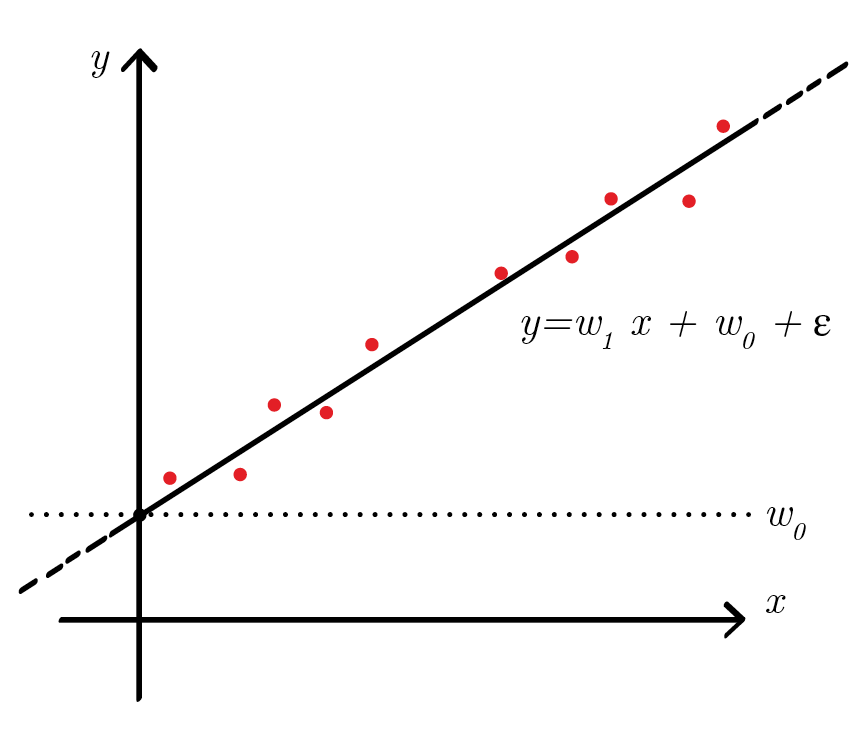
\includegraphics[width=0.5\textwidth]{chapters/intro.regression/figures/2_3.png}
	\caption{\textbf{Probabilistic Model:} Modeling sample noise in the responses. Each sample is now found at $\left(\x_i,y_i\right)$ for $y_i\sim\Nc\left(\x_i^\top \w,\sigma^2\right)$}
\end{figure}

As our model allows some uncertainty in the responses, even for identical $\x$s, we may end up with different $y$s. Let us adapt our learning algorithm from the deterministic case, and deal with the probabilistic (noisy) one. In the same manner as before, using the linear hypothesis class $\Hreg$,  we asusme there exists an unknown coefficients vector $\w$. Denoting the noise vector $\eps=\left(\eps_1,\ldots,\eps_m\right)^\top$ we have in matrix notation: 
\begin{equation}
\y=\X\w+\eps, \quad\quad \eps\sim\Nc\left(0_d,\sigma^2I_d\right)
\label{eqn:lin_reg_prob_model2}
\end{equation}



\paragraph{Geometric Interpretation}
To understand what is the meaning of the sample noise and what will the linear regression model do to the data, let us adapt a geometric interpretation. For $\X\in\R^{m\times d}$ the regression design matrix consider the space spanned by the columns of $\X$. Denote this subspace by $\mathcal{S}\coloneqq Col\left(\X\right) = Im\left(\X\right)$ and consider the OLS solution: $$ \widehat{w} = \left(\X^\top\X\right)^{-1}\X^\top \y $$

For the predicted response vector $\widehat{\y}$ one of the following occurs:
\begin{itemize}
	\item $\widehat{\y}\in\mathcal{S}$: This means that there exists a vector $\w\in\R^d$ such that $\X\w = \y$.
	\item $\widehat{\y}\in\mathcal{S}^\perp$: In this case $\x^\top\y=0$.
	\item $\widehat{\y}$ is a combination of both. Namely we can write $\widehat{\y}$ as some combination $\widehat{\y}=\y_{\mathcal{S}} + \y_\perp$ where $\y_{\mathcal{S}} \in \mathcal{S}$ and $\y_\perp\in\mathcal{S}^\perp$.
\end{itemize}

For the third case we can then express $\widehat{\y}$ as:
\begin{equation}
\begin{array}{ccl}
	\widehat{\y} & =  & \y_{\mathcal{S}} + \y_\perp \\
	& = & \X\w + 0 \\
	& = & \X \left(\X^\top\X\right)^{-1}\X^\top \y
\end{array}
\end{equation}

Where the matrix $\X \left(\X^\top\X\right)^{-1}\X^\top$ is in-fact the \textbf{orgothonal projection matrix} onto the subpsace $\mathcal{S}$. Therefore, the additional sample noise is the component in the response that ``pulls`` $y_i$ out of the subspace. When we perform the linear regression we project the samples onto the estimated subspace and remove the component estimated to be in the perpendicular subspace.  

\begin{figure}[!h]
	\centering
	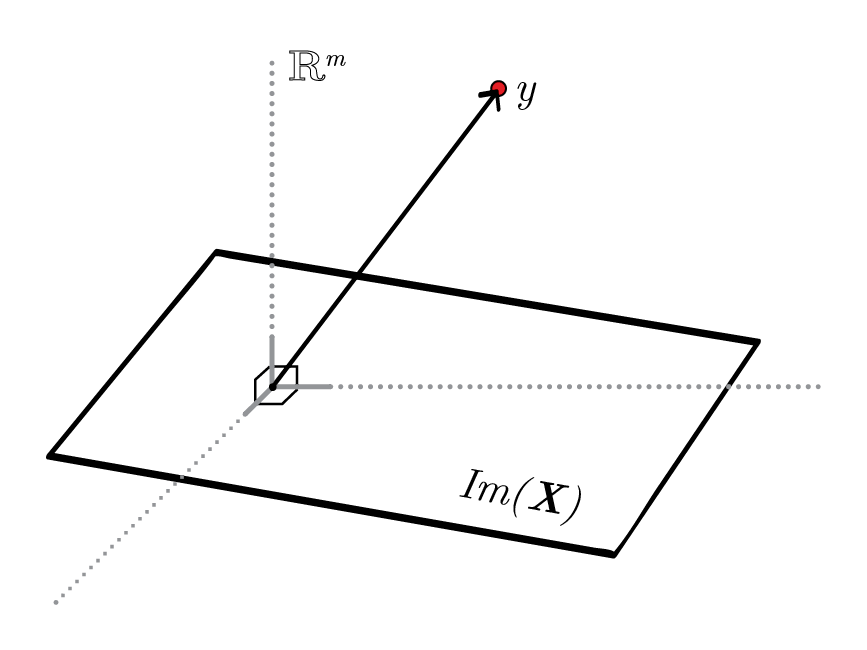
\includegraphics[width=0.45\textwidth]{chapters/intro.regression/figures/2_4.png}
	\hfill
	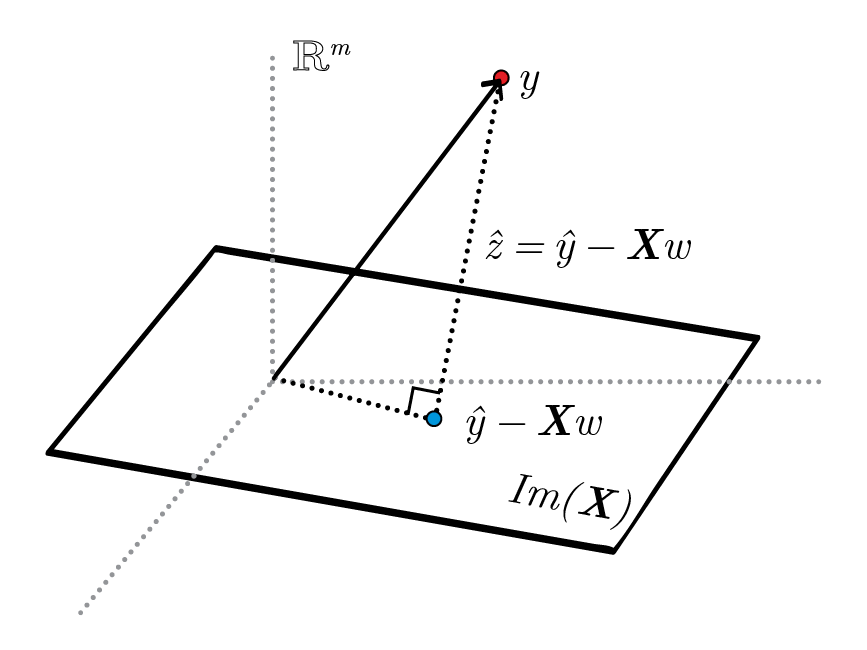
\includegraphics[width=0.45\textwidth]{chapters/intro.regression/figures/2_5.png}
	\caption{\textbf{Linear Regression As Orthogonal Projection:} \todo{add caption}}
	\label{fig:regression_geometric}
\end{figure}


\subsection{Maximum Likelihood Equivalence}
As seen above, different assumptions on the noise in our data yields different traits we can use for our advantage. Let us assume Gaussian noise $\eps\iid\Nc\left(0,\sigma^2\right)$. This means that the $i$-th observation is independently distributed $y_i\sim\Nc\left(\x_i^\top\w,\sigma^2\right)$. Suppose we \textbf{knew} the weight vector $\w$, we could then ask the following question: Given a fixed design matrix $X$ and known coefficients vector $\w$, how likely is it to observe the response vector $\y$?

As we assumed Gaussian noise, we could answer this question using the density function of the Gaussian distribution. %TODO - link to gaussian density
Therefore, the \textbf{likelihood} of $\w$, given the data is:

$$
\begin{array}{ccl}
L\left(\w|X,\y\right) & = & \Prob\left(y_{1}=\x_{1}^{\top}\w,\ldots,y_{m}=\x_{m}^{\top}\w|\X,\w\right) \\
& \overset{iid}{=} & \prod_{i=1}^{m}\Prob\left(y_{i}=\x_{i}^{\top}\w|\X,\right) \\
& = & \prod_{i=1}^{m}\frac{1}{\sqrt{2\pi\sigma^{2}}}\exp\left(-\frac{\left(\x_{i}^{\top}\w-y_{i}\right)^{2}}{2\sigma^{2}}\right) \\
& = & \frac{1}{\left(2\pi\sigma^{2}\right)^{m/2}}\prod_{i=1}^{m}\exp\left(-\frac{\left(\x_{i}^{\top}\w-y_{i}\right)^{2}}{2\sigma^{2}}\right)\\
& = & \frac{1}{\left(2\pi\sigma^{2}\right)^{m/2}}\exp\left(-\frac{1}{2\sigma^{2}}\sum_{i=1}^{m}\left(\x_{i}^{\top}\w-y_{i}\right)^{2}\right)
\end{array}
$$

So solving for $\w$:
$$ 
\begin{array}{ccl}
\quad\quad\quad\widehat{\w} & = & \underset{\w}{argmax}L\left(\w|\y\right) \\
& = & \underset{\w}{argmax}\log L\left(\w|\y\right) \\
& = & \underset{\w}{argmax}\exp\left(-\frac{1}{2\sigma^{2}}\sum_{i=1}^{m}\left(\x_{i}^{\top}\w-y_{i}\right)^{2}\right) \\ 
& = & \underset{\w}{argmin}\sum_{i=1}^{m}\left(\x_{i}^{\top}\w-y_{i}\right)^{2}
\end{array}
$$

we conclude that the MLE (assuming Gaussian noise) is just the OLS estimator we obtained using the ERM principle over the squared loss. %TODO - link to equation

\subsection{Model Interpretation}
Suppose we fitted a model $\w$ to a regression problem $\X,\y$ with the noise assumptions seen in \ref{eqn:lin_reg_prob_model2}. So:
$$
\begin{array}{ll}
\y=\X\w+\eps & \eps \sim\Nc\left(0,\sigma^2I_d\right)\\
\widehat{\w} = \left[\X^\top\X\right]^{-1}\X^\top\y &
\end{array}
$$
Let us think 


\todo{Matan}
\todo{Begin with simple OLS. change in x -> expected (!) change in y}
\todo{Interpretation in multivariate OLS}
\todo{What can we learn from sign and scale of coefficients - and in general that scale of data matters}


\subsection{Categorical Variables}

Consider the following problem. Suppose we want to predict the price of a house based on the following set of explanatory variables:
\begin{itemize}
	\item The `House Size` is a numeric variable accepting positive numbers.
	\item The `Garden Size` is a categorical variable accepting the values: $small$, $medium$ and $large$.
	\item The `Number of Bedroons` is a categorical numeric variable accepting natural numbers.
	\item The `House Type` is a categorical variable accepting the values: $private\,house$, $apartment$ and $studio-apartment$.
\end{itemize}

~\\We would like to construct the following regression problem: $$ y=\x^\top \w,\quad \w=\left[\begin{array}{l}w_{\text{house size}}\\ w_{\text{garden size}}\\ w_{\text{number of bedrooms}}\\ w_{\text{house type}}\end{array}\right] $$
Notice that we have different \textit{types} of variables, and it is not clear how to treat each one of them. The `House Size` and `Number of Bedrooms` variables are \textit{quantitative} variables where we have a natural order over the values. That is, we are able to state if one house is larger than another or if the number of bedrooms in a house is less than the number of bedrooms in another house. For these variables, solving the set of linear equations seen in a linear regression problem is something we know how to do.

~\\In the case of the `Garden Size` variable, though the values are in fact not numeric ($small$, $medium$ and $large$), we are able to define a logical order over these values. It makes sense to state that $small < medium < large$ or that $large \neq small$. We can think of this order as some encoding of the non-numeric categories as numbers, with the order defined over these numbers being the order of the variable. For example: $small\mapsto 1, medium \mapsto 2, large \mapsto 3$.

~\\Last, consider the `House Type` variable. Can we define some logical map as we did for the `Number of Bedrooms` variable? Are we able to state that in some sense that $studio-apartment > private-house$ or that $studio-apartment < private-house$? As we cannot find any logical ordering we must devise a different manner in which to deal with these variables. The most commonly used method is to encode these categories in what is known as \textit{dummy variables} or \textit{one-hot encoding}. Given a categorical variable with $K$ categories we instead represent it as a binary vectors with $K$ entries, where only one of these entries is ``on``. $$ \x_{\text{house type}} = `apartment` \quad \Rightarrow \quad \x =
\left[\begin{array}{c} x_1\\ x_2\\ x_3 \\ x_4 \\ x_5 \\ x_6 \end{array}\right] \begin{array}{l}\text{house size}\\ \text{garden size}\\ \text{number of bedrooms}\\ \text{private-house}\\\text{apartment} \\ \text{studio-apartment} \end{array}
$$
where $x_4+x_5+x+6 = 1, \,\,x_4,x_5,\x_6\in\left\{0,1\right\}$. 

\begin{remark}
Notice that by converting a single categorical variable with $K$ categories to a one-hot encoding we are in-fact adding $K-1$ variables to our model. This addition has both influences on running times (as the algorithms we use are often polynomial in the number of features) and on the number of samples needed for learning (as we will see in \todo{add reference to sample complexity}).
\end{remark}
\begin{remark}
\todo{add about one-hot creating features that are not independent from one another. and reference to regularization that this is tricky}
\end{remark}

\section{Polynomial Fitting}

Let us expand the model of linear regression. Suppose that instead of modeling the linear relation between $\Xc$ and $\Yc$ as $y=\x^\top\w+\eps$ we introduce a set of functions $h_1,\ldots,h_k$ such that $h_j:\R^d\rightarrow\R^k$. We then define the relation as: $$y_i=\sum_{j=1}^kh_j\left(\x\right)^\top\w_i$$

These functions $h_1,\ldots,h_k$, that are referred to as \textit{basis functions}, enable us to describe a relation that is \textbf{linear in the parameters} $\w$ but could be non-linear in the original input $\x$. One specific case is of polynomial fitting. Let $x_1,\ldots,x_m\in\R$ and $y_1,\ldots,y_m\in\R$. We would like to describe a polynomial relation between $\Xc$ and $\Yc$, of degree at most $k\in\N$. The hypothesis class is: 
\begin{equation}
\Hc^k_{poly}=\left\{x\mapsto p_{\w}\left(x\right)| \w\in\R^{k+1}\right\}
\label{eqn:poly_reg}
\end{equation}
where $p_{\w}\left(x\right)=\sum^{K}_{i=1}w_i x^i$. In this case, we define the set of basis functions to be $h_j\left(x\right)=x^j$ for any $j\in\left\{0,\ldots,k\right\}$. Then denote $h\left(x\right)\coloneqq\left(h_0\left(x\right),\ldots,h_k\left(x\right)\right)^\top$. Thus, a polynomial of degree $k$ is given by:
$$ p_{\w}\left(x\right)=\sum^k_{j=0}h_j\left(x\right)\w_j= \left\langle h\left(x\right),\w\right\rangle =h\left(x\right)^{\top} \w $$

As before we want to find a coefficients vector $\w$. Given a sample $\trainset$ we transform it to a sample $\widetilde{S}\coloneqq\left\{\left(h\left(x_i\right),y_i\right)\right\}^m_{i=1}$, and solve the following LS problem: $$ \widehat{w}\coloneqq\underset{\w\in\R^{k+1}}{argmin}\frac{1}{m}\sum^m_{i=1}\left(h\left(x_i\right)^\top \w -y_i\right)^2 $$

Notice that the design matrix $\X$ defined over the transformed data is the Vandermonde matrix:
$$
\X =
\left[
\begin{array}{ccc}
\horzbar & h\left(x_1\right) & \horzbar \\
\horzbar & h\left(x_2\right) & \horzbar \\
& \vdots    & \\
\horzbar & h\left(x_m\right) & \horzbar
\end{array}
\right] = 
\left[
\begin{array}{ccccc}
1 & x_1 & x_1^2 & \cdots & x_1^k \\
1 & x_2 & x_2^2 & \cdots & x_2^k \\
\vdots & \vdots & \vdots & \vdots & \vdots \\
1 & x_m & x_m^2 & \cdots & x_m^k
\end{array}
\right]
$$

Since we assume that the $x_i$'s are different from one another, the design matrix $\X$ is of full rank. This means that solving this linear (in $\w$) system of equations can be done as we have seen for the non-singular case above.

\begin{remark}
Here we have seen polynomial fitting where $\Xc=\R$. With very little adaptation, we could also allow the input data to be $\Xc=\R^d,\,\,d>1$. In such cases the defined polynomial could include terms of multiplication of two (or more) features. We will encounter such an example in \ref{kernel_method}.
\end{remark}

\begin{figure}[!h]
	\centering
	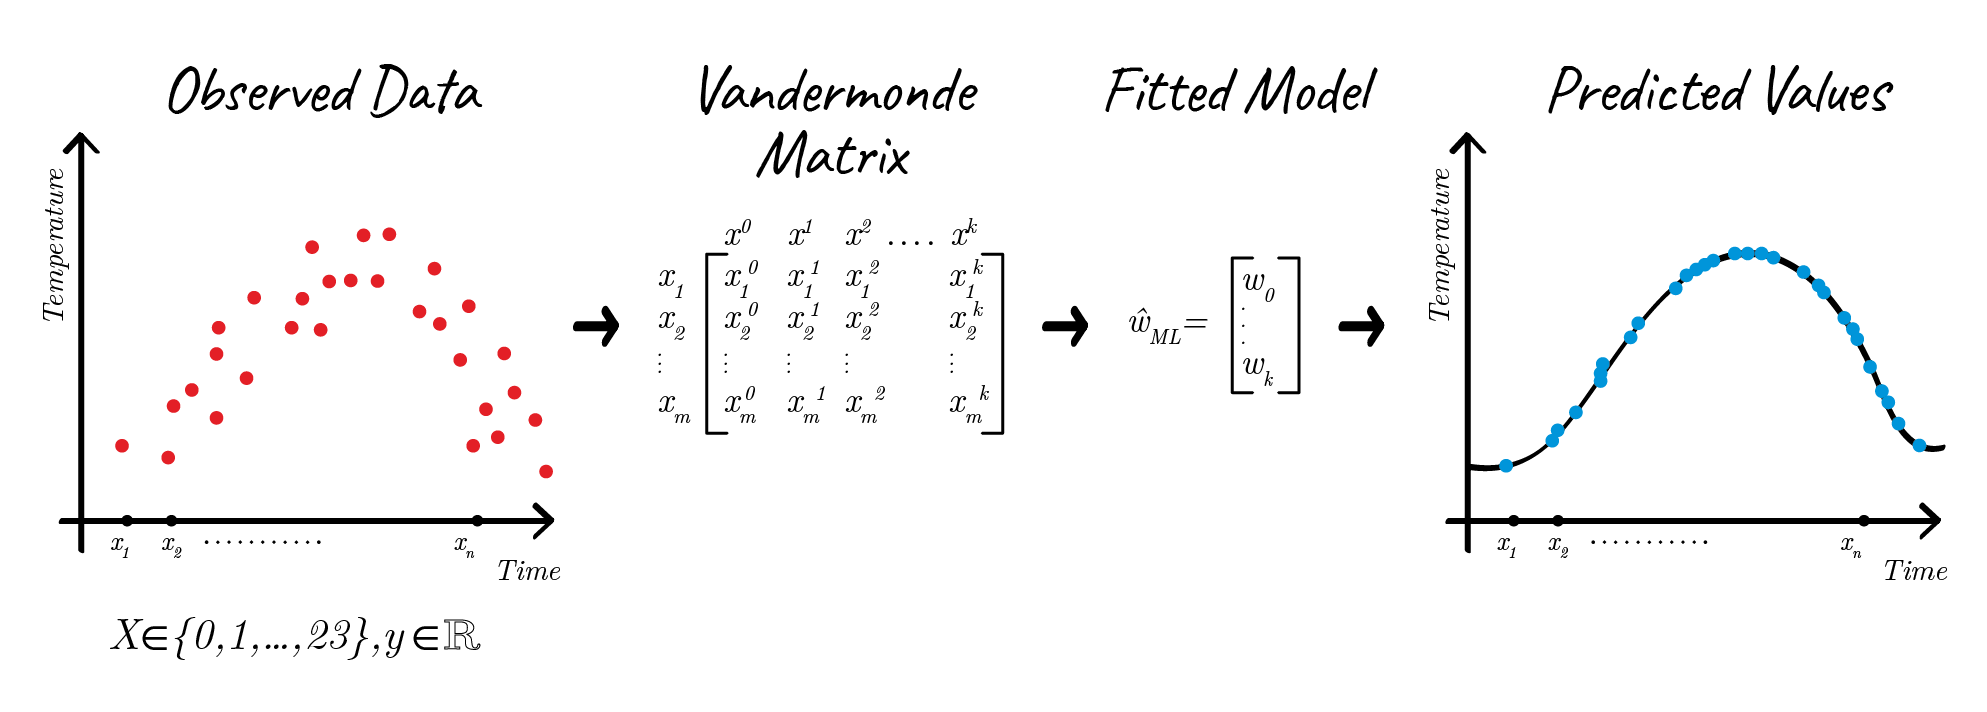
\includegraphics[width=1\textwidth]{chapters/intro.regression/figures/2_6.png}
	\caption{\textbf{Scheme of Polynomial Fitting:} Dataset of hourly temperature where $x_i$ denotes time of day and $y_i$ the temperature. Fitting polynomial of degree $4$.}
\end{figure}


\section{Bias and Variance of Estimators}
Given a regression problem $\X,\y$ we have seen how to solve $\y=\X\w+\eps$. That is, finding a vector $\w$ that satisfies: $\y\approx\X\w$. We showed that the vector minimizing the sum of square distances is given by $$ \ols = \left[\X^\top\X\right]^{-1}\X^\top\y $$
As $\y$ is a random variable, the $\ols$ estimator is a random variable. Therefore, we could look at different properties of such estimator. Specifically, we will look at the \textit{bias} and \textit{variance} of an estimator.
~\\

\begin{definition}\label{eqn:est_bias}
Let $\widehat{\theta}$ be an estimator of $\theta$. The \textit{bias} of $\widehat{\theta}$ is the expected deviation between $\theta$ and the estimator: $B\left(\widehat{\theta}\right)\coloneqq\E\left[\widehat{\theta}\right]-\theta$. $\widehat{\theta}$ is said to be \textit{unbiased} if $B\left(\widehat{\theta}\right)=0$.
\end{definition}

\begin{definition}\label{eqn:est_var}
Let $\widehat{\theta}$ be an estimator of $\theta$. The \text{variance} of $\widehat{\theta}$ is the expected value of the squared sampling deviations: $var\left(\widehat{\theta}\right)\coloneqq\E\left[\left(\widehat{\theta}-\E\left[\widehat{\theta}\right]\right)^2\right]$.
\end{definition}

What is the expectation in both the bias (\ref{eqn:est_bias}) and the variance (\ref{eqn:est_var}) been calculated over? An estimator is a function over a sample $S=x_1,\ldots,x_m\in\R^d$ used to estimate some parameter: $\widehat{\theta}\left(x_1,\ldots,x_m\right)\overset{?}{\approx}\theta$. As such, the expectation of $\widehat{\theta}$ is over the selection of the samples. Going back to the $\ols$ estimator, we could ask what is it's bias and variance.

\begin{exercise}
Let $\X,\y$ be a regression problem such that $\y=\X\w+\eps,\,\,\eps\sim\Nc\left(0,\sigma^2I_d\right)$ and $\widehat{\w}$ being the OLS estimator. Show that $\widehat{\w}$ is an unbiased estimator.
\end{exercise}
\begin{proof}
$$
\begin{array}{ccl}
\E\left[\widehat{\w}\right] & = &\E\left[\left[\X^\top\X\right]^{-1}\X^\top\y\right] \\
& = & \E\left[\left[\X^\top\X\right]^{-1}\X^\top\left(\X\w +\eps\right)\right] \\
& = & \E\left[\left[\X^\top\X\right]^{-1}\X^\top\X\w\right] + \E\left[\left[\X^\top\X\right]^{-1}\X^\top\eps\right]\\
& = & \E\left[\w\right] + \left[\X^\top\X\right]^{-1}\X^\top\E\left[\eps\right] = \w\\
\end{array}
$$
where the last equality is because $\E\left[\eps\right]=0$ and $\w\in\R^d$.
\end{proof}
~\\

To get some intuition about these two properties, let us revisit polynomial fitting. Consider the polynomial $y=x^4-2x^3-0.5x^2+1+\eps$ for $\eps\sim\Nc\left(0,2\right)$. In \autoref{anim:poly1} we choose a set of $x$ values and create 10 different datasets from this model, keeping the $x$ values consistent between datasets but sampling the noise each time: $\left\{\left\{\left(\x_i, y\left(\x_i\right) + \eps_{ij}\right)\right\}^m_{i=1}\right\}^10_{j=1},\,\, \eps_{ij}\iid\Nc\left(0,2\right)$. Then, we fit a polynomial of degree $1$. Black, red and blue points represent the true model, the observed data-points (with the sample noise) and the fitted model over the observed data-points. Notice how the different datasets yield different predicted models. This is the randomness of the prediction, driven by the randomness of the trainset. Over these datasets we can now ask, for each value of $x$, what is the average prediction and its variance:\\
\begin{itemize}
	\item In green is the average prediction of $y$ for a given $x$ across all datasets. The difference between the green and black lines capture the concept of the bias.
	\item In grey is the area of $\E\left[\widehat{y}\right]\pm 2\cdot Var\left(\widehat{y}\right)$ for a given $x$, also known as the confidence interval. The wider this area is, the more out prediction of $\widehat{y}$ varies for different samples. This area captures the concept of the variance.
\end{itemize}

\begin{figure}[h!]
	\centering
	\animategraphics[loop,autoplay,width=0.55\textwidth]{1}{chapters/intro.regression/figures/poly-deg1-diff-samples-}{0}{9}
	\caption{\textbf{Polynomial Fitting:} Fitted polynomial of degree $1$ over different datasets differing only in values of added sample noise. \GitChapterTwoExamples}\label{anim:poly1}
\end{figure}

Two phenomena are visible. The first is that the average distance of the fitted model (in green) and the true model (in black) is large. This means that our hypothesis class doesn't have sufficient expressive power to learn the true model. As such, we conclude that the \textbf{bias} of our estimator is high. The second is that the fitted models over different datasets do not differ by much. As such, we conclude that the \textbf{variance} of our estimator is low.\\

~\\Next, consider the same setup as before but with the fitting of a polynomial of degree $8$ (\autoref{anim:poly8}). This time the different between the average prediction at each $x$ and the true value of $x$ is lower, while the differences between the fitted models (as indicated by the confidence intervals) is much higher. So the \textbf{bias} is low and the \textbf{variance} is high. As we enable more ``flexible`` (i.e. complex) models we are able to fit a model better to our given sample. However, as seen in \autoref{anim:poly8}, if the model is too complex we might actually be fitting a model to the noise, rather than the actual true signal. 
\begin{figure}[h!]
	\centering
	\animategraphics[loop,autoplay,width=0.55\textwidth]{1}{chapters/intro.regression/figures/poly-deg8-diff-samples-}{0}{9}
	\caption{\textbf{Polynomial Fitting:} Fitted polynomial of degree $8$ over different datasets differing only in values of added sample noise. \GitChapterTwoExamples}\label{anim:poly8}
\end{figure}

\begin{remark}
It is important to note that what is seen in the figures are not the bias and variance of $\ols$ themselves but how these manifest over the shown datasets. \todo{refer to relevant labs and chapters}
\end{remark}
~\\
Interestingly, these two properties of bias and variance are linked. Let $\widehat{\y}=\widehat{\y}\left(S\right)$ denote the estimator of $\y$ when using $\ols$, and $\y^*$ the true $\y$ values. When solving the regression problem we wanted to minimize the mean square error between $\widehat{\y}$ and $\y^*$. What would be the expected MSE value?
\\~\\
Denote $\overline{\y}=\E\left[\widehat{\y}\right]$ so:
$$
\begin{array}{ccl}
\E\left[\left(\widehat{\y}-\y^*\right)^2\right] & = & \E\left[\left(\widehat{\y} - \overline{\y} + \overline{\y} -\y^*\right)^2\right] \\
& = & \E\left[\left(\widehat{\y}-\overline{\y}\right)^2\right] + 2\left(\widehat{\y}-\overline{\y}\right)+\left(\overline{\y}-\y^*\right)^2\\
& = & \E\left[\left(\widehat{\y}-\overline{\y}\right)^2\right] + \left(\overline{\y}-\y^*\right)^2\\
& = & var\left(\widehat{\y}\right) + B\left(\widehat{\y}\right)^2
\end{array}
$$
Namely, we could \textbf{decompose} the generalization error (expected square loss between prediction and true value) into a variance component and a (squared) bias component. This means, that whenever we devise some estimator over our training data, the generalization error is influenced by both these factors. This is called the \textbf{Bias-Variance Trade-off}.

\todo{Add proof of variance?}